\documentclass{article}

\usepackage{fontspec}
\usepackage{hyperref}
\usepackage{graphicx}
\usepackage{booktabs}
\usepackage{fancyhdr}
\usepackage{color}
\usepackage{indentfirst}
\usepackage{xeCJK}
\usepackage[hmargin=1.25in,vmargin=1in]{geometry}

\setmainfont{PingFang SC Light}

\title{ST2094-40 HDR 10 plus}
\author{Jiayun Zou}
\date{}
\graphicspath{{images/}}

\begin{document}

\maketitle
\thispagestyle{empty}
\newpage

\tableofcontents
\thispagestyle{empty}
\newpage

\setlength{\parindent}{2em}

\section{Overview}
\begin{figure}[h]
    \centering
    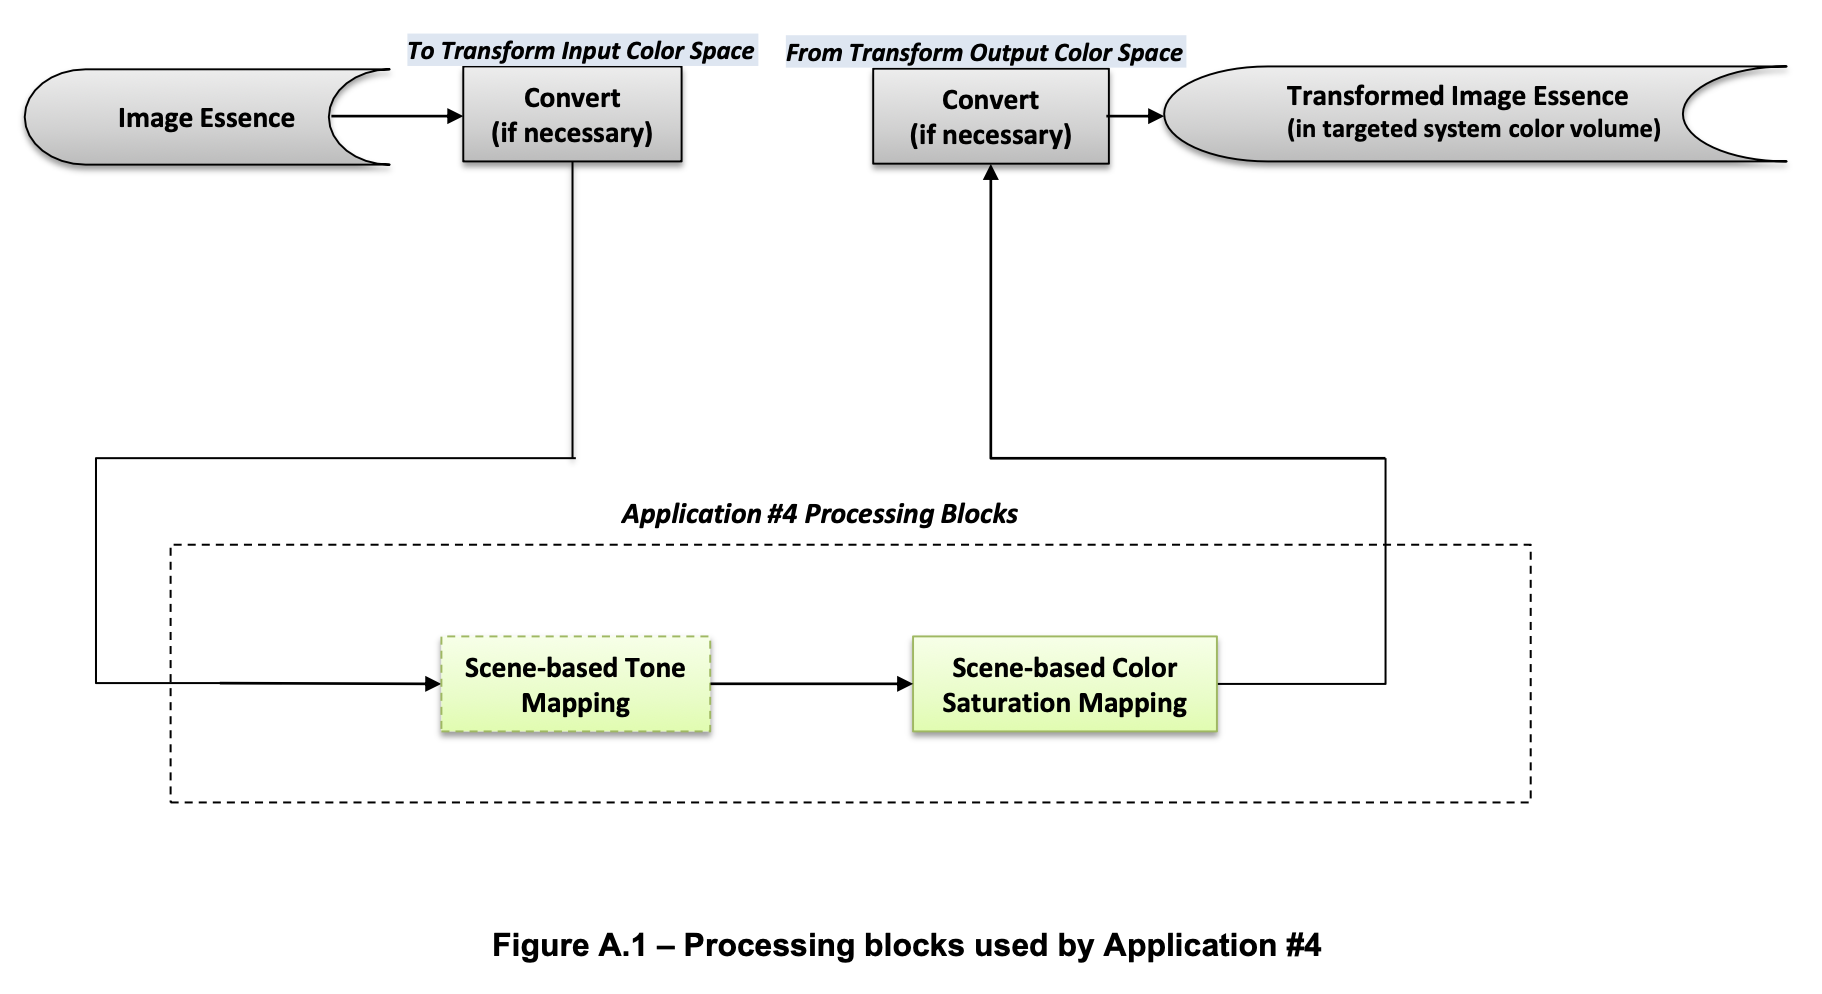
\includegraphics[width=12cm,height=8cm]{Figure1.png}
\end{figure}
Overview \cite{DMfCVTA4}


\section{Metadata Set}\
\begin{table}[h]
    \centering
    \resizebox{\linewidth}{!}{
    \begin{tabular}{l|l|*{2}{l}}
        \toprule
        \multicolumn{2}{c}{Metadata Item} & \multicolumn{2}{c}{Conformance}  \\
        \midrule
        ApplicationIdentifier && \begin{tabular}{l}shall\end{tabular} & \begin{tabular}{l}4\end{tabular} \\
        ApplicationVersion && \begin{tabular}{l}shall\end{tabular} & \begin{tabular}{l}0 or 1\end{tabular} \\
        \midrule
        TimeInterval &\begin{tabular}{l}TimeIntervalStart\\TimeIntervalDuration\end{tabular}&\begin{tabular}{l}shall one\end{tabular}& \\
        \midrule
        ProcessingWindow &\begin{tabular}{l}UpperLeftCorner\\LowerRightCorner\\WindowNumber\\ \midrule CenterOfEllipse \\ RotationAngle \\ SemiMajorAxisInternalEllipse \\ SemiMinorAxisExternalEllipse \\ SemiMajorAxisExternalEllipse \\ OverlapProcessOption\end{tabular}&\begin{tabular}{l}shall one \\ \\ \\ \midrule shall zero or one \\ \\ \\ \\ \\ \\\end{tabular}&\begin{tabular}{l} window 0 shall be always present \\ and shall cover all pixels \\shall be a maximum of 3 \\ \midrule shall be extened with \\ an elliptical pixel selector \\ if Window 1 and 2 is present \\ \\ \\ \\ \end{tabular} \\
        \midrule
        TargetedSystemDisplay &\begin{tabular}{l}TargetSystemDisplayMaximumLuminance \\ TargetedSystemDisplayActualPeakLuminance \end{tabular}&\begin{tabular}{l} shall one \\ shall zero or one \end{tabular}& \begin{tabular}{l} \\ shall/should not include \end{tabular} \\
        \midrule
        ColorVolumeTransform &\begin{tabular}{l} MaxSCL \\ AverageMaxRGB \\ DistributionMaxRGB \\ FractionBrightPixels \\ \midrule MasteringDisplayActualPeakLuminance \\ \midrule KneePoint \\ BezierCurveAnchors \\ \midrule ColorSaturationWeight \end{tabular}&\begin{tabular}{l} shall one \\ \\ \\ \\ \midrule shall zero or one \\ \midrule shall zero or one \\ shall if KneePoint is prsent \\ \midrule shall zero or one \\ \end{tabular}& \begin{tabular}{l} \\ \\ \\ \\ \midrule should/shall not include\\ \midrule \\ \\ \midrule should/shall not include\\ \end{tabular} \\
        \bottomrule
    \end{tabular}}
\end{table}

\subsection{ApplicationVersion}
\noindent \textbf{ApplicationVersion = 0} aims to maintain compatibility with the 2016 edition

- 对OverlapProcessOption方法的规范性描述

- MaxSCL=(0,0,0)不参与计算

- 在DistributionMaxRGB.percentages中,在99处使用99.98对应的百分比

- FractionBrightPixels建议值为0,代表不参与计算

- Bezier曲线增加了Ks=0和Ks=1的计算情况

- \textbf{\textcolor{red}{不建议}}使用某些可选项,\textbf{\textcolor{red}{不建议}}WindowNumber>0

\noindent \textbf{ApplicationVersion = 1} addresses new constraints or requirements

- DistributionMaxRGB有9个位置的累积分布曲线,在99处使用99.98对应的百分比

- BezierCurveAnchors有10个值(不包括0和1),10阶Bezier曲线

- \textbf{\textcolor{red}{禁止}}一些可选项,以及WindowsNumber>0的情况

- FractionBrightPixels有新的计算方法

\subsection{WindowNumber}
在一帧图像中,最多支持3个 Processing Window,其中,Processing Window 0 是必须的,覆盖整个图像,Window 1 和 2 只能够使用椭圆扩展

\subsection{Distribution MaxRGB}
当Metadata中不存在Bezier曲线时,为色调映射提供替代依据

\subsection{Actual Peak Luminance}
在标准中\textbf{\textcolor{red}{不建议}}(ApplicationVersion=0)使用,或者\textbf{\textcolor{red}{禁止}}(ApplicationVersion=1)
在2016版本标准中,附件C提供了Actual Peak Luminance的测量方法,但在2020版本中被删除,如下:


\subsection{FractionBrightPixel}
在2020版本的标准中提供了计算方法,但这应该是视频制作端使用的,并且由于标准中\textbf{\textcolor{red}{不建议}}或者\textbf{\textcolor{red}{禁止}} Actual Peak Luminance,因此FractionBrightPixel也是\textbf{\textcolor{red}{不建议}}或者\textbf{\textcolor{red}{禁止}}的。

\subsection{ColorSaturationWeight}
\textbf{\textcolor{red}{不建议}}(AppliactionVersion=0)甚至\textbf{\textcolor{red}{禁止}}(ApplicationVersion=1),即实际上不建议使用标准中提供的饱和度调整方案。

\section{Scene-based Color Volume Mapping Method}

\subsection{Source Normalized Actual Peak Luminance}
$$M_P = M_{RP} \times S_{MC} \times 10000 / M_{ML}$$
其中,$M_{RP}$为Mastering DisplayActual PeakLuminance,对应2D LUT,输入为$F_{BP}$和$S_{MC}$,分别对应Fraction Bright Pixels和Average MaxRGB,$S_{MC}$为$max(MaxSCL)$,$M_{ML}$为ST 2086中定义的Maximum Display Mastering Luminance。

\subsection{Target Normalized Actual Peak Luminance}
$$T_P = T_{RP} \times S_{MC} \times 10000 / T_{ML}$$
其中,对应系数替换成Target System Display参数。
\subsection{Color Components Normalization}
\begin{equation}
    \left[ \begin{array}{c}
        R_{norm} \\ G_{norm} \\ B_{norm}
    \end{array} \right]
    = \left\{ \begin{array}{cc}
        \min(\left[ \begin{array}{c} 1 \\ 1 \\ 1 \end{array} \right],\frac{1}{M_{RP}}\times \left[ \begin{array}{c} R_{linear} \\ G_{linear} \\ B_{linear} \end{array}\right]), \vspace{0.5ex} & M_{RP} \mbox{ available} \\
        \min(\left[ \begin{array}{c} 1 \\ 1 \\ 1 \end{array} \right],\frac{1}{S_{norm}}\times \left[ \begin{array}{c} R_{linear} \\ G_{linear} \\ B_{linear} \end{array}\right]), & \mbox{ otherwise} 
    \end{array} \right.
\end{equation}

\subsection{Scene Adaptive Tone Mapping}
\begin{equation}
\left[ \begin{array}{c} R_{stm} \\ G_{stm} \\ B_{stm} \end{array} \right] = \min(\left[ \begin{array}{c} 1 \\ 1 \\ 1 \end{array}\right],\frac{F_N(s)}{s}\left[\begin{array}{c} R_{norm} \\ G_{norm} \\ B_{norm} \end{array} \right])
\end{equation}


\subsection{Scene-based Color Saturation Mapping}
饱和度调整是将图像转换到非线性域调整,但标准中设计的调整方案是Local的,即具体的饱和度调整与像素颜色、亮度和Tone-mapping曲线等参数相关,每个像素理论上都可以有不同的饱和度系数,具体的求解方法如下所示:
\begin{equation} f_{scsm}(s) = 1 + \mbox{ColorSaturationweight} \times \max(0, \frac{\log(M_P \times M_{ML} \times s)}{\log(T_P \times T_{ML} \times F_N(s))}-1) \end{equation}

如果$M_P$和$T_P$不存在,则忽略它们(这里理解当Actual Peak Luminance不存在时,则当作默认值1)。同时,标准中给出了饱和度调整的上限计算方法,如下所示:

\begin{equation}
\begin{array}{c} 
    0 <= M_{11} \times Y'_{stm} + \eta (M_{12}C'_{B,stm} + M_{13}C'_{R,stm}) <= 1\\
    0 <= M_{21} \times Y'_{stm} + \eta (M_{22}C'_{B,stm} + M_{23}C'_{R,stm}) <= 1 \\
    0 <= M_{31} \times Y'_{stm} + \eta (M_{32}C'_{B,stm} + M_{33}C'_{R,stm}) <= 1 \\
    0 <= \eta <= 4
\end{array}
\end{equation}

即最终的饱和度调整系数为:

\begin{equation} S_{scsm} = \min(f_{scsm}, \eta) \end{equation}

调整饱和度是在\textbf{\textcolor{red}{非线性域}},因此还需要从线性域转换到非线性域,如下:

\begin{equation}
\left[\begin{array}{c}R_{scsm}\\G_{scscm}\\B_{scsm}\end{array} \right] = EOTF_{1886} M_{2020} \left[ \begin{array}{ccc} 1 & 0 & 0 \\ 0 & S_{scsm} & 0 \\ 0 & 0 & S_{scsm} \end{array} \right] Q_{2020} OETF_{1886} \left[ \begin{array}{c} R_{stm}\\G_{stm}\\B_{stm} \end{array} \right]
\end{equation}

因为这里$S_{scsm}$的计算,需要用到线性域数据,而饱和度调整在非线性域,因此标准中的方案不能够完全放在非线性域计算。

\subsection{Processing Window With Elliptical Pixel Selector}

当椭圆选择窗口存在时,Tone Mapping只对椭圆中的像素进行处理。

\newpage
\bibliographystyle{IEEEtran}
\bibliography{Library}

\end{document}